% SEng 5852 - Spring 2013 White Paper Review
\documentclass{article}
\usepackage{graphicx}

\title{
Exploring the Open Source Process
\\[2\baselineskip]
A Review of \\``A Case Study of Open Source Software Development: The Apache Server''
\\[2\baselineskip]
SEng 5852 - Spring 2013 White Paper Review
\\[2\baselineskip]
}
\author{Kevin Peterson\\
\small \texttt{pete1968@umn.edu}
}

\date{Feb 8, 2013}

\begin{document}
\maketitle


\begin{abstract}
my abstract
\end{abstract}

\section{Introduction}

\section{Methods}

\section{Results}

\section{Data}
\begin{table}
\caption{Table My Table}
\begin{center}
\begin{tabular}{rrrrrrr}
\hline
\hline
Variable & Mean & Min & Max & Std. Dev. \\ 
\hline
Issues  &  30.93  &  1  &  860  &  83.18  \\
Commits  &  249.3  &  1  &  45379  &  1700.01  \\
Closed Issues  &  26.6  &  1  &  837  &  77.56  \\
Open Issues  &  11.37  &  1  &  316  &  31.63  \\
Issue Close Time  &  26.48  &  0  &  503  &  56.54  \\
Issue Creators  &  10.61  &  1  &  128  &  22.29  \\
Committers  &  4.8  &  1  &  405  &  16.39  \\

\hline
\end{tabular}
\end{center}
\end{table}

\section{Acknowledgments}

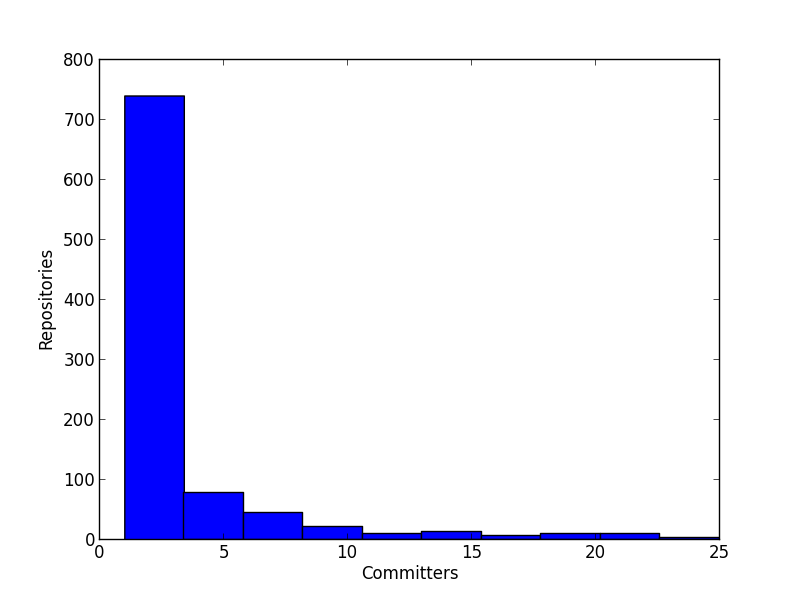
\includegraphics[height=4in,width=4in]{images/committers_histogram.png}

\section{Reviewed Article}
In``A Case Study of Open Source Software Development: The Apache Server''\cite{mockus2000case}, the authors examine the popular Open Source Software (OSS) project Apache Server.\footnote{http://httpd.apache.org/} The article defines six research questions which it answers after an examination of the project. These questions examine the process, team makeup, and general quality of the software produced in order to determine if an OSS project can compete with commercially developed equivalents. This review summarizes the authors' key points, as well as includes my analysis and summary.

\section{Article Key Points}

\subsection{OSS Process} The development process of Apache does not include many of the traditional Software Engineering components, such as project plans, schedules, or even formal design -- attributes it shares with many OSS projects\cite{dibona1999open}. Despite this, many OSS projects (including Apache) are thought to be of equal or higher quality than commercial equivalents.\\
Although there is no defined process, a process does emerge organically. Problems are typically reported through a USENET mailing list. After a problem or new feature has been identified, how development progresses depends heavily on the ideas of a {\it developer hierarchy} and {\it code ownership}. In absence of a dedicated Quality Assurance (QA) team, or even defined system-testing phases, {\it quality and support} is a distributed, community undertaking.

\subsection{Developer Hierarchy} Apache is built around a small set of {\it Core Developers}, followed by {\it Defect Repairers} and {\it Defect Reporters}. Each level of this hierarchy brings with it an order of magnitude increase in number of participants. The 10-15 {\it Core Developers} contribute around 80\% of the new functionality, while the rest of the 400 code contributors focus primarily on bug fixes. The {\it Defect Reporters} were by far the largest group, with over 3000 individuals submitting bug reports.
   
\subsection{Code Ownership} {\it Core Developers} rely on mutual trust in each other's expertise to avoid having to strictly partition the code base to avoid conflicts. If this expertise and trust is sufficient, {\it Core Developers} do not need to segment or limit commit rights amongst themselves. The set of core developers is surrounded by ``satellite'' groups, which then own the development of additional functionality. As stated in the article, this effectively breaks the OSS project into a collection of related OSS projects. This is necessary because a small core of developers has a natural limit to their code output.

\subsection{Quality and Support} Given the same amount of testing, OSS will have a lower defect density than commercial software. There are several reasons for this. Notably, most OSS is written by passionate domain experts. Also, given the sheer number of people that review changes, defects are more likely to be caught without having to go through formal testing cycles. Regarding customer support, a rapid response to problems can be obtained because OSS is not bound to release schedules in the same way commercial software is. ``Patches'' may be released at any time, by any member of the community.

\section{Analysis of Key Points}

\subsection{OSS Process}
The authors suggest pairing these OSS ideas with a more structured commercial software process, and I find that idea very interesting. I am not convinced that simply ``evolving'' without a high level design or project plan is advisable, even though there are success stories. I am unsure as to whether it is {\it in spite of} or {\it because of} the process that this project was successful. There seems to be very real limitations in this process, such as code base size. The idea of the ``community as an asset'' is well described as very useful in reviewing code and finding defects.

\subsection{Developer Hierarchy}
Skill and experience of developers is one of the key factors in OSS quality\cite{hedberg2007assuring}. If OSS can be the vehicle that brings together a talented core of domain experts, that in itself is an accomplishment regardless of process. Also, participation expands as the amount of potential impact decreases -- which is a logical but interesting point. Bug reporters, for example, do not have to be necessarily trusted with core functionality, but can still contribute a valuable service -- and there can be many of them.
   
\subsection{Code Ownership}
Collective code ownership is an important part of the Extreme Programing (XP) process, and I believe is generally useful regardless of process or software license. It is interesting that lacking a defined process, OSS comes to the same conclusion on this point as XP, as XP explicitly lists collective code ownership as one of their core values\cite{beck1999embracing}.

\subsection{Quality and Support}
Quality is governed by the group as a whole, primarily through mailing list discussions and the opportunity for any change/patch to be reviewed by the community. This peer scrutiny, along with the pride of work that comes with working in a domain that the contributors are passionate about, are highlighted as important factors in a lower (pre-test) defect count. However, I believe that the intrinsic reward\cite{lakhani2003open} felt by many from supporting OSS projects will be a challenge to duplicate in commercial offerings.

\section{Summary}
OSS development, as mentioned in the article, is its own unique process. It is interesting to see, given a set of developers and a shared project, the process that evolves. A process that has evolved organically (as opposed to one dictated by management) can perhaps give us a better understanding of how we as Software Engineers really work.\\
The article shows that even though the OSS process may appear to be unstructured and unorganized, in reality roles and hierarchies appear. This structure may be organically created -- but is structure none the less.\\
I believe that the ideas of Code Ownership were highlighted especially well in this article. The authors conclude that these ideas are successful because of shared respect for experience and ability. This point is powerful, and something that all processes should strive for.\\
Data analysis was also done comparing Apache to several similar commercial products. This data helps to confirm the hypotheses of the authors, and makes a very strong argument for the viability of this process.





  
\bibliographystyle{plain}
\bibliography{bibliography}




\end{document}
